\chapter{Kehitysympäristö Vagrantilla}

\section{Ongelma}
Yleinen ongelma usean kehittäjän tiimissä on kehitysympäristöjen erilaisuus. Tämä ilmenee parhaiten kun kehittäjät käyttävät työkoneellaan eri käyttöjärjestelmiä kuten Linuxia, OS X:ää ja Windowsia. Usein projekteihin sisältyy pitkät asennusohjeet, jossa kerrotaan tarkasti mitkä riippuvuudet pitää asentaa sekä niiden tarkat versionumerot. Usein riippuvuuksien asennus on erilaista riippuen käyttöjärjestelmästä. Ei ole epätavallista, että ympäristön pystytykseen voi mennä muutama työpäivä. Oman kokemukseni mukaan pystytysprosessiin menee paljon henkilötyötunteja, sillä lähes aina projektiin tullut uusi kehittäjä tarvitsee apua projektissa aikaisemmin olleilta henkilöiltä.

\section{Ratkaisu}
Yksi ratkaisu saada samanlaiset kehitysympäristöt ohjelmoijille on käyttää virtuaalikoneita. VirtualBox tai WMware ovat esimerkkejä virtuaalikoneohjelmista. Virtuaalikoneet ovat täysiverisiä käyttöjärjestelmiä isäntäkoneen eli kehittäjän koneen sisällä. Usein kehityskäyttöjärjestelmäksi valitaan jokin Linux paketti esimerkiksi Ubuntu. Näin kaikille kehittäjille saadaan sama käyttöjärjestelmä, jossa kehitys tapahtuu. Tämä vähentää riippuvuuksien asentamisessa tapahtuvaa virheiden määrää.

Käyttöjärjestelmien yhdenmukaistaminen ei yksistään riitä, sillä ongelmat ilmenevät usein riippuvuuksien asentamisessa. Pelkkä VirtualBoxin lisäksi tarvitaan muita ohjelmia, koska muuten halutut ohjelmat pitää asentaa käsin tai tehdä iso kokoinen levykuva, josta ympäristö asennettaisiin.

\section{Vagrant}
Vagrantin avulla voidaan luoda virtuaalikoneita helposti komentoriviltä. Se on yksinkertainen ohjelma, joka ainoastaan antaa komentoja VirtualBoxille. Tästä syystä VirtualBox täytyy olla asennettuna, jotta Vagrant toimii.

Vagranttia kannattaa ajatella vertauskuvan kautta. Kuvitellaan, että Erik haluaa perustaa Subway-ravintolan. Koska Subway on pikaruokaravintolaketju sillä on tarkasti määritelty muun muassa mitä aineksia ruoka-annoksissa saa käyttää, miten ravintola sisustetaan ja minkälaiset laitteisto täytyy olla.

Erik saa itse valita tilan, johon ravintola perustetaan. Tilan valitsemisen jälkeen hänen täytyy sisustaa ravintola Subwayn määrittämällä tavalla. Seuraavaksi täytyy hankkia uuni, jääkaappi ja muut ruuan tekemiseen tarkoitetut välineet. Tässä vaiheessa saattaa tulla tilanne, jossa kaikki hankitut laitteet eivät välttämättä sovi valittuun liiketilaan. Esimerkiksi Erikin valitsemalle jääkaappille ei välttämättä löydy sopivaa paikkaa. Yhteensopivuus ongelmia voi syntyä ennen kuin uusi Subway-ravintola voidaan avata. Tämä on luonnollista, koska Subwayn johto ei voi tietää miten kaikki laitteet asettuvat mihin tahansa liiketilaan.

Kun Subwayn liikejohto huomasi, että uusilla ravintoloiden perustajilla on usein ongelmia ravintolan pystyttämisessä ja sen saamiseksi ohjeiden mukaiseen kuntoon he päättivät helpottaa asiaa. He kehittivät uusien ravintoloiden perustajille paketin, josta täytyy vain painaa nappia eikä ravintoloitsijan tarvitse tehdä muuta. Erik kokeili uutta asennuspakettia ja huomasi, että paketista tuli ulos robotti, joka lähti heti rakentamaan liiketilaa ravintolalle. Robotti rakentaa aina samanlaisen tyhjän liiketilan johdon määrittelemällä tavalla. Kun liiketila on valmis robotti aloittaa jääkaappien, uunien ja muiden laitteiden asentamisen, jotka ovat välttämättömiä Subway-ravintolan pitäjälle. Kun laitteet ovat asennettu liiketila viimeistellään sisustuksella. Robotti tiesi miten asennukset ja sisustaminen pitää tehdä, koska sille on määritelty ohje, jota se lukee. Kun robotti on tehnyt kaiken se antaa liiketilan avaimet Erikille, jonka ei tarvitse muuta kuin laittaa uunit päälle niin hän voi aloittaa myymisen.

Vertauskuvassa liiketila on kehittäjän oma tietokone. Liiketilaan halutaan saada Subway-ravintola, joka edustaa tiettyä koodausprojektia. Subway ravintolalla on tiettyjä määrityksiä siitä minkälainen sen pitäisi olla. Ravintolan määritykset kuvaavat koodausprojektin riippuvuuksia kuten tietokantaohjelmistoa ja sen versiota. Kehitysympäristön käsiasennusta kuvataan, kun Erik asentaa itse laitteita liiketilaan.

Paketti, joka sisältää robotin kuvastaa automatisoitua kehitysympäristöä. Kun robotti luo liiketilan tyhjästä tarkoitetaan virtuaalikoneen luomista isäntäkoneen sisälle.

\subsection{Vagrantin toiminta}
Vagrant luo isäntäkoneen sisälle virtuaalikoneen kuten kuvassa \ref{fig:how-vagrant-works}. Virtuaalikone sisältää kaikkille kehittäjille yhteinen käyttöjärjestelmän. Lisäksi Vagrantille annetaan "resepti", jonka mukaan se asentaa kaikki projektin riippuvuudet virtuaalikoneelle. Koodin kääntäminen, komentojen ajaminen, mahdollisen tietokannan käyttäminen tms. asiat tehdään virtuaalikoneella. Näin isäntäkone pysyy puhtaana turhista ohjelmista, eikä synny aikaisemmin mainittuja ongelmia. Isäntäkoneessa tapahtuu koodin kirjoittaminen, tiedostojen luonti ja versionhallinan käyttäminen.

Kun uusi kehittäjä liittyy tiimiin hänen tarvitsee vain kloona repositorio, mennä projektin kansioon ja komentaa \code{vagrant up}. Muutaman hetken päästä uudella kehittäjällä täydellinen kehitysympäristö, joka on täysin samanlainen kaikkien tiimin kehittäjien kanssa. Uusi kehittäjä käyttää isäntäkonetta vain koodaamisessa. Projektin koodit synkronoidaan virtuaalikoneelle Vagrantin avustuksella. Näin kehittäjä voi käyttää tuttua käyttöjärjestelmää haluamillaan ohjelmilla, jotka liittyvät koodin tuottamiseen. Samalla säilyttäen saman ajo- ja käännösympäristön kuin muilla kehittäjillä.

\begin{figure}[h]
  \includegraphics[width=\textwidth]{how-vagrant-works}
  \caption{Vagrantin toiminta isäntäkoneen sisällä}
  \label{fig:how-vagrant-works}
\end{figure}

\subsection{Vagrantin käyttäminen}
Ennen Vagrantin käytön aloittamista täytyy VirtualBox ja Vagrant olla asennettuna. Vagranttia käytetään terminaalin kautta. Asennus on onnistunut, jos komento \code{vagrant -v} palauttaa versionumeron.

Siirry projektikansioon ja aja \code{vagrant init}. Vagrant luo kansioon Vagrantfile-nimisen tiedoston. Vagrantfile on käytännössä Ruby-ohjelmointi kieltä, jota Vagrant osaa lukea kun se ajetaan. Vagrantfilessä voi siis käyttää kaikkia Ruby-kielen toimintoja. Kuviosta \ref{listing:InitialVagrantfile} näkyy tiedoston sisältö ilman kommentteja.

\begin{lstlisting}[
  label=listing:InitialVagrantfile,
  language=Ruby,
  caption=Alustava Vagrantfile,
  float=h
]
Vagrant.configure(2) do |config|
  config.vm.box = "ubuntu/trusty64"
end
\end{lstlisting}

Kaikki virtuaalikoneen asetukset tulevat config-osion sisälle. Tällä hetkellä koneelle määritellään vain boxi: "ubuntu/trusty64". Mahdollisia boxeja voi etsiä osoitteesta: \url{https://atlas.hashicorp.com/boxes/search}. Boxit ovat käytännössä käyttöjärjestelmä eli pohja virtuaalikoneelle. Tässä tapauksessa boxina on Ubuntu, joka perustuu Debian Linux-jakeluun \cite{link:ubuntu}. Boxi on ravintolavertauskuvassa ravintolan liiketila. Boxi on pakko olla, mutta itsessään sillä ei tee paljon mitään. Boxi täytyy \enquote{sisustaa} eli asentaa projektiin liittyvät ohjelmat ja riippuvuudet.

Yksinkertaisin keino asentaa ohjelmia virtuaalikoneelle on shell-skriptien avulla. Jos projektiin tarvitsee asentaa vain muutama ohjelma voidaan ne asentaa laittamalla asennus-skripti suoraan Vagrantfileen. 

\begin{lstlisting}[
  label=listing:vagrant-shell-inline,
  language=Ruby,
  caption=Vagrantin yksinkertainen shell-skripti,
  float=h
]
config.vm.provision "shell",
  inline: "apt-get update; apt-get install -y apache2"
\end{lstlisting}

Kuviossa \ref{listing:vagrant-shell-inline} Vagrantfilen sisään on lisätty provisiointi shell-skripti, joka on tyyppiä inline. Tällä tarkoitetaan, että koko skripti annetaan suoraan stringinä. Tässä esimerkissä \code{apt-get update} päivittää virtuaalikoneen lokaalit pakettilinkit. \code{apt-get install -y apache2} tarkoittaa että asennetaan Apache-palvelinohjelma, jota monet käyttävät esimerkiksi PHP-projekteissa. Lippu -y pitää lisätä, koska apt varmistaan usein käyttäjältä, että haluaako hän varmasti asentaa kyseisen paketin. Lippu varmistaa sen, että kaikki pakettiin liittyviin kysymyksiin vastataan kyllä.

Skripti voidaan myös jakaa monelle riville Rubyn HEREDOC:n avulla kuvion \ref{listing:vagrant-shell-heredoc} osoittamalla tavalla. HEREDOC \cite{link:ruby-heredoc} mahdollistaa stringin kirjoittamisen monelle riville, mikä helpottaa luettavuutta kun asennetaan paljon ohjelmia.

\begin{lstlisting}[
  label=listing:vagrant-shell-heredoc,
  language=Ruby,
  caption=Vagrantin shell-skripti HEREDOC:lla,
  float=h
]
config.vm.provision "shell", inline: <<-SHELL
  apt-get update
  apt-get install -y apache2
SHELL
\end{lstlisting}

Käytännössä kuitenkin shell-skripti kannattaa laittaa erilliseen tiedostoon kuten kuviossa \ref{listing:vagrant-shell-path}. Skriptin nimeäminen riittää, jos Vagrantfile ja shell-skripti ovat samassa kansiossa.

Ulkoiseen skriptii täytyy laittaa alkuun kommentti, jossa kerrotaan, että kyseessä on shell-skripti. Ulkoisen skriptiin on helppo määritellä paljon eri ohjelmien asennuksia ja konfigurointeja.

\begin{lstlisting}[
  label=listing:vagrant-shell-path,
  language=Ruby,
  caption=Provisiointi-skripti voi olla myös erillisessä tiedostossa,
  float=h
]
config.vm.provision "shell", path: "install-environment.sh"
\end{lstlisting}

\begin{lstlisting}[
  label=listing:vagrant-external-shell-script,
  language=bash,
  caption=Ulkoinen shell-skripti,
  float=h
]
#!/bin/bash
apt-get update
apt-get install -y apache2
\end{lstlisting}

Ohjelmointi tehdään isäntäkoneella, joten olisi käytännöllistä saada siitä suora yhteys virtuaalikoneelle asennettuihin ohjelmiin. Tilanteessamme Apache on esimerkki tällaisesta ohjelmasta. Siksi seuraavaksi pitää avata virtuaalikoneen portteja host-koneelle. Apache vastaa oletuksena osoitteesta \url{http://localhost:80}, joten haluamme avata portin 80 isäntäkoneelle. Vagrantfileen voidaan määrittää mikä virtuaalikoneen portti halutaan ohjata mihin isäntäkoneen porttiin. Kuviossa \ref{listing:vagrant-port-mapping} virtuaalikoneen portti 80 ohjataan isäntäkoneen porttiin 8080.

\begin{lstlisting}[
  label=listing:vagrant-port-mapping,
  language=Ruby,
  caption=Virtuaalikoneen portti 80 ohjataan isäntäkoneen porttiin 8080,
  float=h
]
config.vm.network "forwarded_port", guest: 80, host: 8080
\end{lstlisting}

Nyt kun isäntäkoneella mennään selaimella osoitteeseen \url{http://localhost:8080} niin pitäisi tulla näkyviin Apachen oletussivu jos Apache on asennettu joillakin edellä mainituilla tavoilla virtuaalikoneeseen. Kuvassa \ref{fig:apache-default-page} näkyy Apachen oletussivu kun virtuaalikoneen portit on ohjattu oikein.

\begin{figure}[h]
  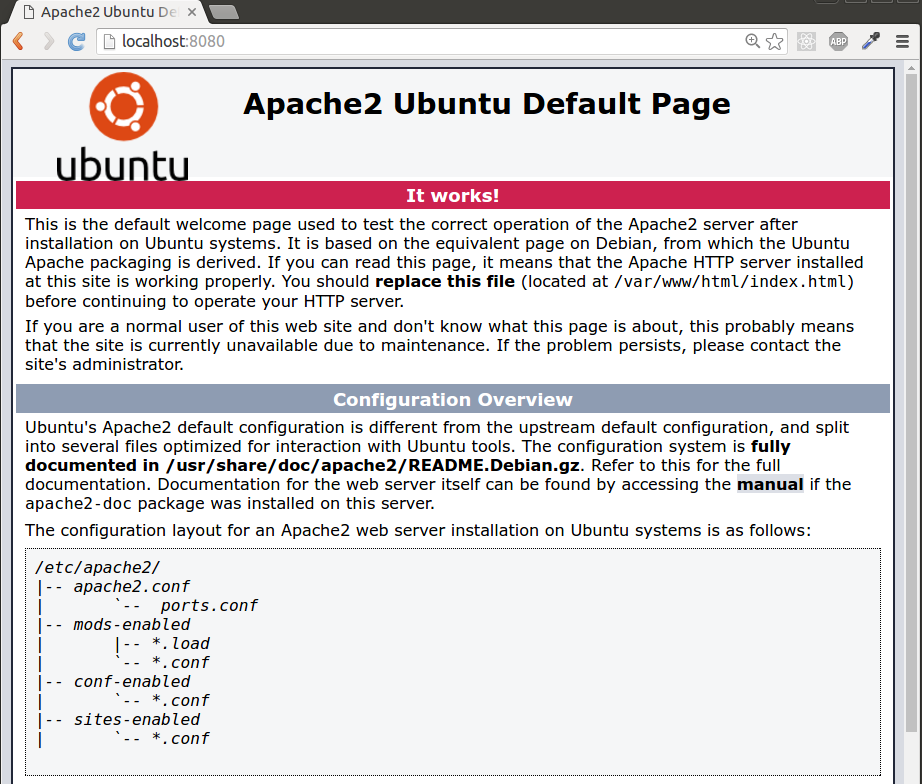
\includegraphics[width=\textwidth]{apache-default-page}
  \caption{Isäntäkone näkee Apachen oletussivun kun oikeat portit ovat auki}
  \label{fig:apache-default-page}
\end{figure}

Nyt kun Apache on asennettu oikein voidaan virtuaalikoneelle viedä projektin tiedostostot. Oletetaan, että projektissa on yksinkertaisuuden vuoksi vain index.html-tiedosto. Kuviossa \ref{listing:vagrant-synced-folder} näytetään miten haluttu kansio saadaan synkronoitua virtuaalikoneeseen. Ensimmäinen parametri kertoo mikä isäntäkoneen kansio halutaan synkronoida. Polun voi antaa relatiivisena tai absoluuttisena. Tässä tapauksessa parametri on relatiivisesti nykyinen kansio. Toinen parametri kertoo minne kansio halutaan synkronoida virtuaalikoneessa. Isäntäkoneen kansio halutaan synkronoida kansioon /var/www/html, koska sieltä Apache lukee oletuksena tiedostoja. Nyt kun lisätään projektin juureen isäntäkoneella tiedosto index.html, jonka sisältönä on \code{Hello from project file} saadaan kuvan \ref{fig:index-file-response} mukainen vastaus Apachelta.

\begin{figure}[h]
  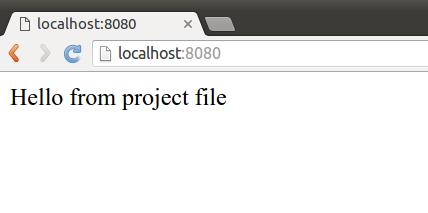
\includegraphics[width=\textwidth]{index-file-response}
  \caption{Apache vastaa index.html tiedoston sisällön}
  \label{fig:index-file-response}
\end{figure}

Vagrant synkronoi tiedostot valittujen kansioiden välillä molempiin suuntiin. Kun tiedosto lisätään isäntäkoneella, sama tiedosto ilmestyy virtuaalikoneelle. Samoin jos virtuaalikoneelle lisätään tiedosto synkronoituun kansioon, tämä tiedosto tulee isäntäkoneelle. Työskennellessä on tarkoitus toimia lisäämällä tiedostoja aina isäntäkoneelle.


Jos isäntä- ja virtuaalikoneella on kaksi saman nimistä tiedostoa, isäntäkoneella oleva tiedosto ylikirjoittaa virtuaalikoneen tiedoston. Esimerkiksi kansiossa /var/www/html on Apachen oletus index.html-tiedosto, mutta projektin index.html ylikirjoittaa sen.

Kuvassa \ref{fig:how-vagrant-works} on visualisoitu kaksisuuntainen kansion synkronointi.

\begin{lstlisting}[
  label=listing:vagrant-synced-folder,
  language=Ruby,
  caption=Isäntäkoneen kansio synkronoidaan virtuaalikoneen kansioon,
  float=h
]
config.vm.synced_folder ".", "/var/www/html"
\end{lstlisting}

\subsection{Vagrantin yhteenveto}

Lopullinen Vagrantfile on kuvion \ref{listing:vagrant-final-apache-setup} mukainen. Vagrantfilessä määriteltiin ensiksi "pohjaboxi", joka määrittelee käyttöjärjestelmän. Seuraavaksi ohjataan virtuaalikoneen portti 80 osoittamaan isäntäkoneen porttiin 8080. Synkronoidaan nykyinen projektikansio Apachen html-juureen. Lopuksi määritellään skripti, joka ajetaan kun virtuaalikone luotu ja käynnistetty ensimmäistä kertaa.

\begin{lstlisting}[
  label=listing:vagrant-final-apache-setup,
  language=Ruby,
  caption=Lopullinen Vagrantfile Apache koneelle,
  float=h
]
Vagrant.configure(2) do |config|
  config.vm.box = "ubuntu/trusty64"

  config.vm.network "forwarded_port", guest: 80, host: 8080

  config.vm.synced_folder ".", "/var/www/html"

  config.vm.provision "shell", path: "install-environment.sh"
end
\end{lstlisting}


Vagrant näyttää ensi silmäyksellä olevan täydellinen ratkaisu kaikille projekteille, on siinä omat huonot puolensa. Vagrant vie paljon isäntäkoneen keskusmuistia, koska se luo täysiverisiä virtuaalikoneita isäntäkoneen sisään. Oman kokemukseni mukaan 8 gigatavua keskusmuistia on riittänyt. Tosin laajemmissa projekteissa, joissa tarkkaillaan satojen tiedostojen muutoksia, voi 8 gigatavua keskusmuistia olla liian vähän. Virtuaalikone kannattaa välillä käynnistää uudestaan, jos isäntäkone käy liian kuumata. Tällaisissa tilanteissa kannattaa harkita keskusmuistin lisäämistä isäntäkoneeseen.

Kannattaa myös miettiä milloin projektille on järkevää lisätä virtuaalikone kehitysympäristöksi. Yleisenä nyrkkisääntönä on, että jos koodia tulee kehittämään useampi kehittäjä, niin virtuaalikoneympäristö kannattaa olla. Myös jos projekti sisältää paljon riippuvuuksia, niin on hyvä miettiä läpi virtuaalikoneesta saatavat hyödyt.

Alle on koottu Vagrantin hyödyt ja mahdolliset haitat.

Vagrantin hyödyt
\begin{bullet-list}
  \item Isäntäkoneelle, ei tarvitse asentaa projektille spesifejä riippuvuuksia.
  \item Projektin kehitysympäristön asennustiedot ovat versionhallinnassa Vagrantfilessä ja skripteissä.
  \item Ympäristön saa helposti pystyyn vain komentamalla \code{vagrant up}.
  \item Kaikilla kehittäjillä sama kehitysympäristö.
\end{bullet-list}

Vagrantin haitat
\begin{bullet-list}
  \item Virtuaalikoneella työskentely vie enemmän keskusmuistia kuin suoraan isäntäkoneella työskentely.
  \item Yleensä tarvitsee tehdä enemmän konfiguraatiota esimerkiksi kun tarkkaillaan tiedostojen muutoksia ja halutaan reagoida niihin.
\end{bullet-list}

\subsection{Vagrantin ongelmat}

Vagrant lupaa kotisivuillaa \cite{link:vagrant}, että se luo identtiset ympäristöt kaikille tiimissä, tätä ei kuitenkaan täysin ongelmitta saavuteta.

Eniten ongelmia tulee, jos isäntäkoneessa on Windows. Yleensä Windowsille tarvitsee tehdä ylimääräisiä säätöjä esimerkiksi kun tiedostoja synkronoidaan isäntäkoneelta virtuaalikoneelle. Vagrantissa oletuksena oleva tiedostojen synkronointi on hidas \cite{link:vagrant-shared-folders} kun synkronoitavana on paljon tiedostoja. Tilannetta voidaan nopeuttaa vaihtamalla synkronointi tavaksi NFS \cite{link:nfs-wiki}. Se on testituloksien mukaan nopeampi. Windows ei tue NFS:ää, mikä kannattaa ottaa huomioon isäntäkonetta valittaessa.

Toinen yleinen ongelma Windowsissa ilmenee, kun projektin riippuvuuksia asennetaan npm:n avulla. Komennettaessa \code{npm install} npm hakee projektin riippuvuudet, jonka jälkeen riippuvuuksien riippuvuudet sitten niiden riippuvuudet ja niin edelleen. Tästä aiheutuu pitkiä tiedostopolkuja, joita Windows ei osaa kunnolla käsitellä. Kuviossa \ref{listing:npm-error-long-path} on esimerkki npm:n virheestä, joka sisältää pitkän tiedostopolun.

Pitkien tiedostopolkujen ongelmaa on ratkaistu muun muassa säätämällä Vagrantin lähdekoodissa synkronoitavien kansioiden käsittelyä \cite{link:fix-npm-on-vagrant-on-windows}. Tai asentamalla riippuvuudet ilman linkkejä \cite{link:npm-does-not-work-in-vagrant}. Yksi paras ratkaisuista on tehdä virtuaalikoneen sisällä symbolinen linkki riippuvuuskansiosta, jolloin Windows ei yritä synkata kansiota isäntäkoneelle, eikä mene sekaisin.

\begin{lstlisting}[
  label=listing:npm-error-long-path,
  language=Ruby,
  caption=Npm virhe jossa pitkä tiedostopolku,
  float=h
]
Error: EPERM, open '/srv/www/harvsworld/htdocs/wp-content/themes/
harvsworld/node_modules/gulp-imagemin/node_modules/imagemin/
node_modules/imagemin-optipng/node_modules/optipng-bin/
node_modules/bin-wrapper/node_modules/download-status/
node_modules/lpad-align/package.json'
\end{lstlisting}

Vaikka Vagrant mahdollistaa kehitysympäristön pystytyksen lähes millä tahansa isäntäkoneella, kannattaa tiimin sisällä olla samat käyttöjärjestelmät. Toiseksi parasvaihtoehto on käyttää unix-pohjaisia käyttöjärjestelmiä. Näin säästytään mahdollisilta lisäsäädöiltä, jotka pääasiassa johtuvat Windowsista.